\documentclass[a4paper,french]{paper}
\usepackage{../../../../../_assets/latex/5N_OPTO_ELEC}

%Informations about this document 
%------------------------------------------
\def\module{Opto-Electronique - S5}
\def\moduleAbrege{5N-027-SCI / OptoElec}
\def\annee{2024-2025}

\def\titre{Séance 2 / Capteurs et mise en forme}
\author{Julien VILLEMEJANE}

\subtitle{Séance 2}
\institution{LEnsE / Institut d'Optique Graduate School}

\title{\titre}
\begin{document} 
%Beginning First Page. 
%------------------------------------------
\enteteThematiqueObligatoire{}

\textit{Pour ce TD, on pourra s'appuyer sur la fiche résumée} : \href{https://lense.institutoptique.fr/ressources/Annee1/Electronique/fiches/2021_FR_ALI.pdf}{Ampli Linéaire Intégré}.

%Beginning Content. 
%------------------------------------------


%%%%%%%%%%%%%%%%%%%
\encadreTDExo{2.1 - Élever une tension}{
Proposez un circuit permettant d'élever une tension d'un facteur $k$.

$k > 1$
}

%%%%%%%%%%%%%%%%%%%
Pour pouvoir élever une tension, il est nécessaire d'\textbf{apporter de l'énergie au montage}. Une solution possible est l'utilisation d'un amplificateur opérationnel (ou amplificateur linéaire intégré - ALI).

On peut par exemple utiliser un montage de type amplificateur non-inverseur dont le schéma est fourni ci-dessous :

\begin{center}
\begin{circuitikz}
	\draw (0,0) node[above]{} to[short, o-, i=$i^+$] ++(1,0)
	node[op amp, noinv input up, anchor=+, fill=blue!10!white](OA){\texttt{AOP1}}
	(OA.-) to[short,-, i<_=$i^-$] ++(0,-1) coordinate(FB)
	to[R=$R_1$, i=$I_1$] ++(0,-2.3) node[ground]{}
	(FB) to[R=$R_2$, *-] (FB -| OA.out) to[short,-, i<_=$I_2$] (OA.out)
	to [short, *-o] ++(1,0) node[above]{};
	\draw (0,-0.3) edge[<-,color={green!40!black}] (0, -4);
	\draw (0,-4.3) to[open,-o] ++(0,0) node[ground](GND){};
	\node[text={green!40!black}] (Ve) at (-0.5,-2.1){$V_E$}; 
	\draw (4.3,-1) edge[<-,color={red}] (4.3, -4);
	\draw (4.3,-4.3) to[open,-o] ++(0,0) node[ground](GND){};
	\node[text={red}] (Vs) at (4.8,-2.7){$V_S$}; 
\end{circuitikz}
\end{center}

Pour pouvoir faire le calcul de la fonction de transfert entre $V_S$ et $V_E$, il est nécessaire de faire \textbf{quelques hypothèses}.

La \textbf{première} vient du fait que les impédances d'entrée de tel amplificateur sont relativement grandes par rapport aux impédances des composants extérieurs ($R_1$ et $R_2$ ici). Les courants d'entrée $i^+$ et $i^-$ peuvent alors être négligés et considérés nuls.

La \textbf{seconde} hypothèse vient ici du fait que l'amplificateur a sa sortie rebouclé avec l'entrée inverseuse (-) par l'intermédiaire d'une résistance. Dans ce cas, on considère que le montage est en \textbf{fonctionnement dit linéaire}. Ainsi, on peut montrer que la différence de potentiel entre $V^+$ et $V^-$ tend vers 0. On peut alors considérer dans ce régime de fonctionnement, que $V^+ = V^-$.

\medskip

Il est alors possible par les lois habituelles de calculer le lien entre $V_S$ et $V_E$.

D'après la première hypothèse, on obtient que $I_1 = I_2$.

D'après la seconde hypothèse, on obtient que $V^- = V_E$.

En calculant le courant $I_1$ par la loi d'Ohm aux bornes de $R_1$, on obtient : $I_1 = \frac{V_E}{R_1}$.

De la même manière, on obtient : $I_2 = \frac{V_S - V_E}{R_2}$.

Après simplification, on obtient alors la fonction de transfert suivante : $$\boxed{V_S = V_E \cdot \frac{R_1 + R_2}{R_1}}$$


\noindent\hrulefill

\textbf{Attention !} Cette loi n'est cependant vraie qu'en basse fréquence et pour des tensions d'entrée faibles.

En effet, les amplificateurs linéaires intégrés sont des composants qui peuvent se modéliser comme un système de type \textbf{passe-bas}.

De plus, ils nécessitent d'être alimentés et lorsque la tension de sortie tend à dépasser la tension d'alimentation, on peut observer un \textbf{phénomène de saturation}.


%%%%%%%%%%%%%%%%%%%
%%%%%%%%%%%%%%%%%%%
\encadreTDExo{2.2 - Amplifier un signal}{
Proposez un circuit permettant d'amplifier un signal de $27dB$, tout en garantissant une bande-passante de $400 kHz$.

On utilisera des amplificateurs linéaires intégrés de type TL081 (documentation partielle donnée en annexe du TD1).
}

%%%%%%%%%%%%%%%%%%%

On souhaite un gain $G_{dB} = 27\operatorname{dB}$.

On rappelle que $G_{dB} = 20 \cdot \log (A)$ avec $A$ l'amplification.

Ainsi $A = 10^{\frac{G_{dB}}{20}} = 22.4$.

\medskip

Le \textbf{produit gain bande-passante est constant} sur un ALI. Dans le cas du \textit{TL081}, il vaut : $GBP = 3\operatorname{MHz}$.

La fréquence de coupure obtenue avec un ALI de type TL081 et une amplification de 22.4 serait : $f_c = \frac{GBP}{A} = 134\operatorname{kHz} < 400\operatorname{kHz}$. 

\textbf{Un seul étage n'est donc pas suffisant.}

\medskip

En mettant plusieurs étages amplificateurs en cascade, les amplifications se multiplient. Ainsi pour 2 étages, si on appelle $K$ l'amplification d'un étage, on obtient alors $A = K^2$.

Chaque étage aura alors une amplification $K = \sqrt{A} = 4.73$. La bande-passante d'un étage sera alors $f_c = \frac{GBP}{K} = 634\operatorname{kHz} > 400\operatorname{kHz}$.

Il faudra alors utiliser 2 étages amplificateurs inverseurs (ou non-inverseurs) dont l'amplification sera de 4.73.

%%%%%%%%%%%%%%%%%%%
%%%%%%%%%%%%%%%%%%%
\encadreTDExo{2.3 - Additionner des signaux}{
On se propose d'étudier le circuit suivant :

\begin{center}
\begin{circuitikz} 
	\node [op amp, fill=blue!10!white](A1) at (0,0){\texttt{AOP1}};
	\draw (A1.-) to[short] ++(-.5,0) coordinate(A) to[short, -*] ++(0,1.5) coordinate(B) to[R=$Z_S$] (B -| A1.out) to[short, -*] (A1.out);
		
	\draw (A1.-) to[short,-*] ++(-.5,0) coordinate(AA) to[R=$Z_1$] ++(-2.5,0) coordinate(BB) to[short,-o] ++(-.5,0) coordinate(CC);
	
	\draw (B) to[R=$Z_i$] ++(-2.5, 0) to[short, -o] ++(-1.5, 0);
	
	\draw (B) -- ++(0, 1.5) to[R=$Z_N$] ++(-2.5, 0) to[short, -o] ++(-2.5, 0);	
	
	\draw (A1.+) to[short] ++(0,-0.5) node[ground]{};
	\draw (A1.out) to[short,-o] ++(1,0) coordinate(D);
	\draw (-4.6,-1) edge[->,color={green!40!black}] (-4.6,0.3);
	\node[text={green!40!black}] (Ve) at (-5.1,-0.35){$V_{e1}$};		\draw (-4.6,-1.3)  to[open,-o] ++(0,0) node[ground](GND){};


	\draw (-5.6,-1) edge[->,color={green!40!black}] (-5.6,1.7);
	\node[text={green!40!black}] (Ve) at (-6.1,0.65){$V_{ei}$};	
	\draw (-5.6,-1.3)  to[open,-o] ++(0,0) node[ground](GND){};
	
	\draw (-6.6,-1) edge[->,color={green!40!black}] (-6.6,3.1);
	\node[text={green!40!black}] (Ve) at (-7.1,1.35){$V_{eN}$};	
	\draw (-6.6,-1.3)  to[open,-o] ++(0,0) node[ground](GND){};
	 
	
	\draw (2.2,-1) edge[->, color={red}] (2.2,-0.3);
	\node[text={red}] (Vs) at (1.7,-0.6){$V_s$}; 
	\draw (2.2,-1.3)  to[open,-o] ++(0,0) node[ground](GND){};
	
\end{circuitikz}
\end{center}
}

On fera les \textbf{hypothèses suivantes} :
\begin{itemize}
	\item \textbf{fonctionnement linéaire}, car rebouclage entre la sortie et l'entrée inverseuse par la résistance $Z_S$, ainsi $V^+ = V^-$ ;
	\item \textbf{amplificateur parfait}, ainsi $i^+ = i^- = 0$. 
\end{itemize}

\medskip

\textbf{Noeud en $V^-$} $I_S + I_1 + I_i + I_n = 0$

\textit{On supposera les courants positifs ceux venant de l'extérieur du montage.}

\medskip

\textbf{Calcul des courants} par la loi d'Ohm

De plus $V^+ = 0$, ainsi $V^- = 0$.

$I_S = \frac{V_S - V^-}{Z_S} = \frac{V_S}{Z_S}$

$I_1 = \frac{V_1 - V^-}{Z_1} = \frac{V_1}{Z_1}$

$I_i = \frac{V_i - V^-}{Z_i} = \frac{V_i}{Z_i}$

$I_n = \frac{V_N - V^-}{Z_N} = \frac{V_N}{Z_N}$

\medskip

Après simplification (et généralisation) on obtient alors :

$$V_{S} = - Z_S \cdot \sum_{i=1}^{N} \frac{V_i}{Z_i} $$



%%%%%%%%%%%%%%%%%%%
%%%%%%%%%%%%%%%%%%%
\encadreTDExo{2.4 - Mettre en forme un capteur de température}{
On se propose d'étudier le circuit suivant :

\begin{center}
	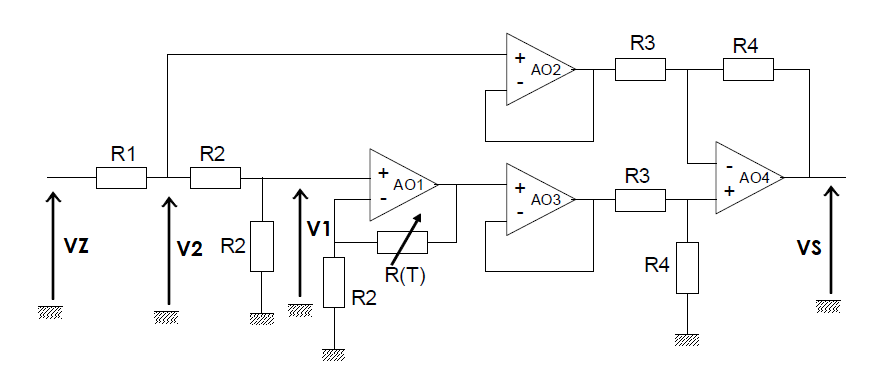
\includegraphics[width=16cm]{images/capteur_conditionnement.png}
\end{center}

La thermistance utilisée est de type PT100. La relation entre sa résistance (en Ohms) et la température (en \degre{}C) est la suivante :
$$R(T) = 100~(1 + 3.908×10^{-3} T - 5.802×10^{-7} T^2)$$
}

%%%%%%%%%%%%%%%%%%%

\textbf{Etude du montage}

Pour étudier ce circuit, on commence par \textbf{décomposer en blocs} plus facilement calculables, en partant du signal de sortie.

De manière générale, chaque amplificateur linéaire (ALI) correspond à un montage particulier. Il peut donc être intéressant d'identifier les montages associés à chaque ALI.

Ici, on peut décomposer de cette façon : 
\begin{itemize}
	\item Autour de l'AO4 : amplificateur différentiel 
	\item Autour des AO2 et AO3 : suiveur / découplage
	\item Autour de l'AO1 : montage linéaire de type amplificateur / tension de sortie dépendante de la température
	\item Autour de la diode Zener : tension de référence	
\end{itemize}


\textbf{AO1} 

Hypothèse classique : fonctionnement linéaire ($V^+ = V^-$) et ALI parfait ($i^+ = i^- = 0$).

$V+ = V_Z \cdot R_2 / (R_1 + 2 R_2)$ et $V- = V_1 \cdot R_2 / (R_2 + R(T))$, alors : 

$$V_1 = V_Z \cdot \frac{R_2}{R_1 + 2 R_2} \cdot \frac{R_2 + R(T)}{R_2} = V_Z \cdot \frac{R_2 + R(T)}{R_1 + 2 R_2}$$

\textbf{AO2} : suiveur / diviseur de tension

$$V_2 =  V_Z \cdot \frac{2 \cdot R_2}{R_1 + 2 R_2}$$

\textbf{AO3} : suiveur

$$V_3 = V_1$$

\textbf{AO4} 

$V- = (V_S/R_4 + V_2/R_3) / (1/R_3 + 1/R_4)$ (Millmann)

$V+ = V_3 \cdot R_4 / (R_3 + R_4)$

On a alors : 

$$V_S = (V_3 - V_2) \cdot \frac{R_4}{R_3}$$


\textbf{Montage complet}

$$V_S = V_Z \cdot \frac{R_4}{R_3} \cdot \frac{R(T) - R_2}{R_1 + 2 R_2}$$

$$V_S = V_Z \cdot \frac{R_4}{R_3} \cdot \frac{R_2}{R_1 + 2 R_2} \cdot (\frac{R(T)}{R_2} - 1)$$


Lorsque $T < 0$, $R(T) < R_2$ et donc $V_S < 0$. Alimentation symétrique indispensable.


%%%%%%%%%%%%%%%%%%%
%%%%%%%%%%%%%%%%%%%
\encadreTDExo{2.B1 - Pilotage TOR en fonction de la luminosité}{

\textit{TOR signifie Tout Ou Rien}

On souhaite réaliser un détecteur qui allume une LED lorsque la luminosité ambiante diminue. On propose pour cela le montage suivant qui utilise une cellule photoconductrice CdS. On donne : $V_{cc} = 12\operatorname{V}$ et $R_2 = 100\operatorname{k\Omega}$.

\begin{center}
	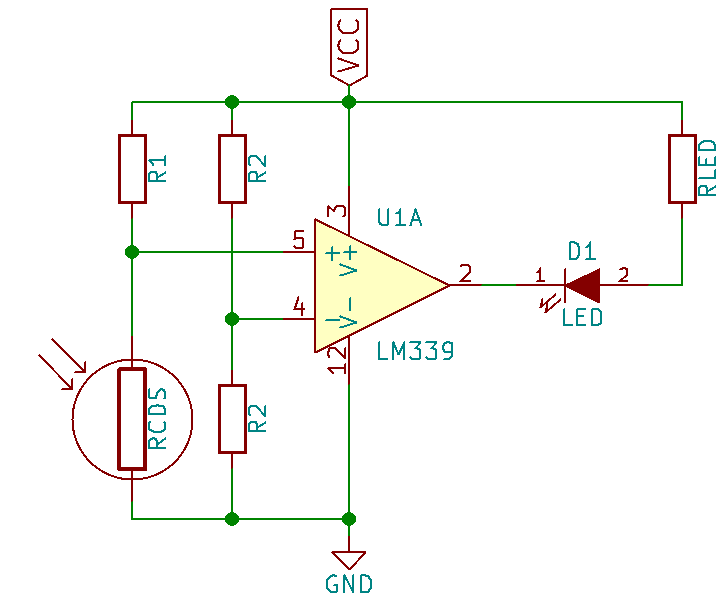
\includegraphics[width=9cm]{images/comparateur_luminosite.png}
\end{center}

On donne ci-dessous les caractéristiques de la cellule CdS.

\begin{center}
	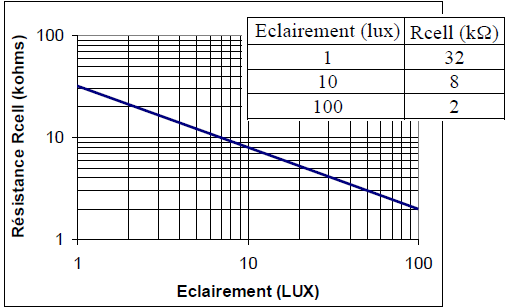
\includegraphics[width=10cm]{images/capteur_CDS.png}
	
	Caractéristique Résistance en fonction de l'Eclairement de la cellule CDS
\end{center}

On rappelle que l'amplificateur linéaire intégré, le \textbf{LM339}, est un comparateur à collecteur ouvert (voir la fiche résumée \textsc{Amplificateur Linéaire Intégré}).

\begin{enumerate}
	\item Quelle est la fonction réalisée par l'amplificateur opérationnel (AO) dans ce montage ?
	\item Dans quelle condition sur $V+$ et $V-$ la LED sera-t-elle allumée ?
	\item Calculer la tension à la sortie de la cellule CDS.
	\item Vérifier le bon fonctionnement du système.

\medskip
	
	On mesure la valeur de la photocellule ($R_{cell0} = 5\operatorname{k\Omega}$) dans des conditions d'éclairement ambiant. 
	
	\item Calculer la valeur de $R_1$ pour que la LED s'allume lorsque l'éclairement diminue d'un facteur 10.
\end{enumerate}
}

%%%%%%%%%%%%%%%%%%%

\textbf{Question 1}

Il n'y a pas de contre-réaction, donc mode \textbf{comparateur} :

\begin{itemize}
	\item si $V+ > V-$ alors passage de courant entre le collecteur ouvert et la masse.
	\item si $V+ < V-$ alors pas de passage de courant entre le collecteur ouvert et la masse.
\end{itemize}

\textbf{Question 2}

\begin{itemize}
	\item Pour allumer la LED, il faut un passage de courant, donc lorsque $V+ > V-$
	\item Pour éteindre la LED, il faut que le courant soit nul, donc lorsque $V+ < V-$
\end{itemize}

Or $V- = V_{CC} / 2$. Lorsque la tension aux bornes de la cellule CDS dépasse $V_{CC} / 2$, on a alors allumage de la LED.

\textbf{Question 3}

$V_{CDS} / V_{CC} = R_C / (R_C + R_1)$

\textbf{Question 4}

\begin{itemize}
	\item Eclairement faible : si $R_C = 10 \cdot R_1$ alors $V_{CDS} / V_{CC} = 10 / 11$
	\item Eclairement limite : si $R_C = R_1$ alors $V_{CDS} / V_{CC} = 1 / 2$ 
	\item Eclairement élevé : si $R_C = R_1 / 10$ alors $V_{CDS} / V_{CC} = 1 / 11$
\end{itemize}

\textbf{Question 5}


D'après la doc technique, la résistance $R_{cell}$ est multipliée par 4 lorsque l'éclairement est divisée par 10

Ainsi, $R_1 = 4 \cdot R_{cell0} = 20 \operatorname{k\Omega}$

\end {document}